\chapter{Исследовательская часть}

В данном разделе будут приведены исследование временных характеристик реализуемых алгоритмов и оценка их затрат по памяти.

\section{Технические характеристики}

Технические характеристики устройства, на котором выполнялись замеры по времени:

\begin{itemize}
    \item Процессор: Intel i5-1035G1 (8) @ 3.600 ГГц.
    \item Оперативная память: 16 ГБайт.
    \item Операционная система: Manjaro Linux x86\_64 (версия ядра Linux 5.15.131-1-MANJARO).
\end{itemize}

Во время проведения измерений времени ноутбук был подключен к сети электропитания и был нагружен только системными приложениями.

\section{Демонстрация работы программы}

На рисунке \ref{fig:prog-demo} демонстрация работы программы для случая, когда пользователь выбирает опцию 1 <<Сортировка массива>> и передает в программу массив $[5, 3, 2, 9, 7]$.

\begin{figure}[H]
    \centering
    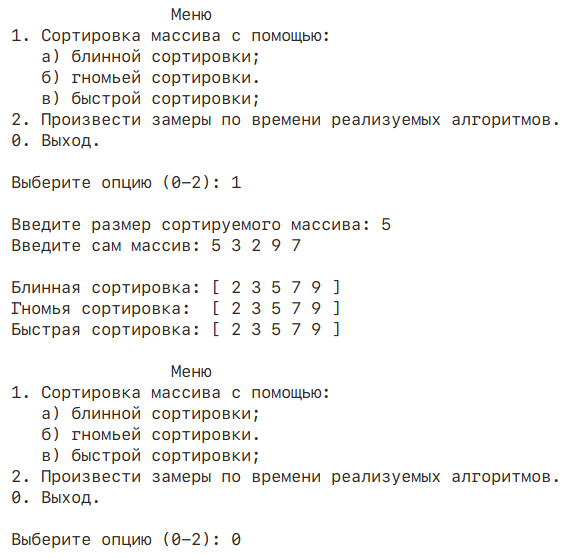
\includegraphics[width=0.8\textwidth]{images/prog_demo.png}
    \caption{Демонстрация работы программы}
    \label{fig:prog-demo}
\end{figure}

\section{Временные характеристики}

Исследование временных характеристик реализуемых алгоритмов производилось три раза:

\begin{enumerate}
    \item на массивах, упорядоченных по возрастанию, размер которых изменяется от 1 до 1001 с шагом 100;
    \item на массивах, упорядоченных по убыванию, размер которых изменяется от 1 до 1001 с шагом 100;
    \item на неупорядоченных массивах, размер которых изменяется от 1 до 1001 с шагом 100;
\end{enumerate}

В силу того, что время работы алгоритмов может колебаться в связи с различными процессами, происходящими в системе, для обеспечения более точных результатов измерения для каждого алгоритма повторялись 100 раз, а затем бралось их среднее арифметическое значение.

На рисунке \ref{fig:forw-time} показаны зависимости времени выполнения блинной, гномьей и быстрой сортировок от размера упорядоченного по возрастанию массива.

На рисунке \ref{fig:backw-time} показаны зависимости времени выполнения блинной, гномьей и быстрой сортировок от размера упорядоченного по убыванию массива.

На рисунке \ref{fig:rand-time} показаны зависимости времени выполнения блинной, гномьей и быстрой сортировок от размера неупорядоченного массива.

\begin{figure}[H]
    \centering
    \includesvg[width=1.0\textwidth]{images/time/forward.svg}
    \caption{Результат измерений времени работы реализуемых алгоритмов на массивах, упорядоченных по возрастанию}
    \label{fig:forw-time}
\end{figure}

\begin{figure}[H]
    \centering
    \includesvg[width=1.0\textwidth]{images/time/backward.svg}
    \caption{Результат измерений времени работы реализуемых алгоритмов на массивах, упорядоченных по убыванию}
    \label{fig:backw-time}
\end{figure}

\begin{figure}[H]
    \centering
    \includesvg[width=1.0\textwidth]{images/time/random.svg}
    \caption{Результат измерений времени работы реализуемых алгоритмов на неупорядоченных массивах}
    \label{fig:rand-time}
\end{figure}

\section{Характеристики по памяти}

Введем следующие обозначения:
\begin{itemize}
    \item $\text{size}(v)$~--- функция, вычисляющая размер входного параметра v в байтах;
    \item $int$~--- целочисленный тип данных.
\end{itemize}

Теоретически оценим объем используемой алгоритмами памяти при сортировке массива размером $N$.


\subsection{Блинная сортировка}

Оценка используемой блинной сортировкой памяти приведена в формуле \ref{eqn:mem-pansort}.

\begin{equation}
    \label{eqn:mem-pansort}
    M_{PanSort} = 6 \cdot \text{size}(int) + N \cdot \text{size}(int) + 8,
\end{equation}
где $5 \cdot \text{size}(int)$~--- размер дополнительных переменных,
\\ $N \cdot \text{size}(int)$~--- размер целочисленного массива,
\\ $8$~--- адрес возврата.

\subsection{Гномья сортировка}

Оценка используемой гномьей сортировкой памяти приведена в формуле \ref{eqn:mem-gnsort}.

\begin{equation}
    \label{eqn:mem-gnsort}
    M_{GnSort} = 3 \cdot \text{size}(int) + N \cdot \text{size}(int),
\end{equation}
где $5 \cdot \text{size}(int)$~--- размер дополнительных переменных,
\\ $N \cdot \text{size}(int)$~--- размер целочисленного массива.


\subsection{Быстрая сортировка}

Оценка используемой быстрой сортировкой памяти приведена в формуле \ref{eqn:mem-qsort}.

\begin{equation}
    \label{eqn:mem-qsort}
    M_{QSort} = M_{call} \cdot
    \begin{cases}
        \log_2{N}, & \text{лучший случай} \\
        N, & \text{худший случай}
    \end{cases}
\end{equation}
где  $M_{call} = (8 + 3 \cdot \text{size}(int) + N \cdot \text{size}(int))$~--- размер памяти, затрачиваемый на один рекурсивный вызов,
\\ $5 \cdot \text{size}(int)$~--- размер дополнительных переменных,
\\ $N \cdot \text{size}(int)$~--- размер целочисленного массива,
\\ $\log_2{N}$~--- глубина стека вызовов в лучшем случае,
\\ $N$~--- глубина стека вызовов в худшем случае,
\\ $8$~--- адрес возврата.

\section*{Вывод}
\addcontentsline{toc}{section}{Вывод}

В результате исследования реализуемых алгоритмов по времени выполнения можно сделать следующие выводы:
\begin{enumerate}
    \item алгоритм быстрой сортировки показал наибольшую скорость выполнения на упорядоченных по убыванию и неупорядоченных массивах (см. рисунки \ref{fig:backw-time}, \ref{fig:rand-time});
    \item на массивах, упорядоченных по возрастанию, наиболее эффективным оказался алгоритм гномьей сортировки (см. рисунок \ref{fig:forw-time}), однако в остальных случаях этот алгоритм показал наименьшую производительность;
    \item на неупорядоченных массивах скорость работы быстрой сортировки выше, чем на упорядоченных.
\end{enumerate}

В результате теоретической оценки алгоритмов по памяти можно сделать вывод о том, что алгоритм гномьей сортировки является наименее ресурсозатратным.
Алгоритм быстрой сортировки, напротив, требует больше всего памяти, что объясняется тем, что алгоритм рекурсивный, и на каждый вызов функции требуется выделение памяти на стеке для сохранения информации, связанной с этим вызовом.